%! Author = itgramic
%! Date = 05.12.23

% Preamble
\subsubsection{Monolithische vs. verteilte SQL Systeme}
\begin{flushleft}
    Klassische SQL-Datenbanken sind Monolithische Systeme, selbst wenn sie mittels Replikation eine Primary/Standby-Architektur aufweisen.
    Man kann mittels eines SQL Proxys ein gewisses Mass an Load Balancing betreiben, hat aber immer noch das Problem das es einen Primary Node gibt auf dem beschrieben wird.
    Monolithische Systeme sind daher nicht Cloud Native.
\end{flushleft}
\begin{flushleft}
    Nur verteilte Systeme, sogenannte Distributed SQL wiederum sind Cloud Native

    \begin{figure}[H]
        \centering
        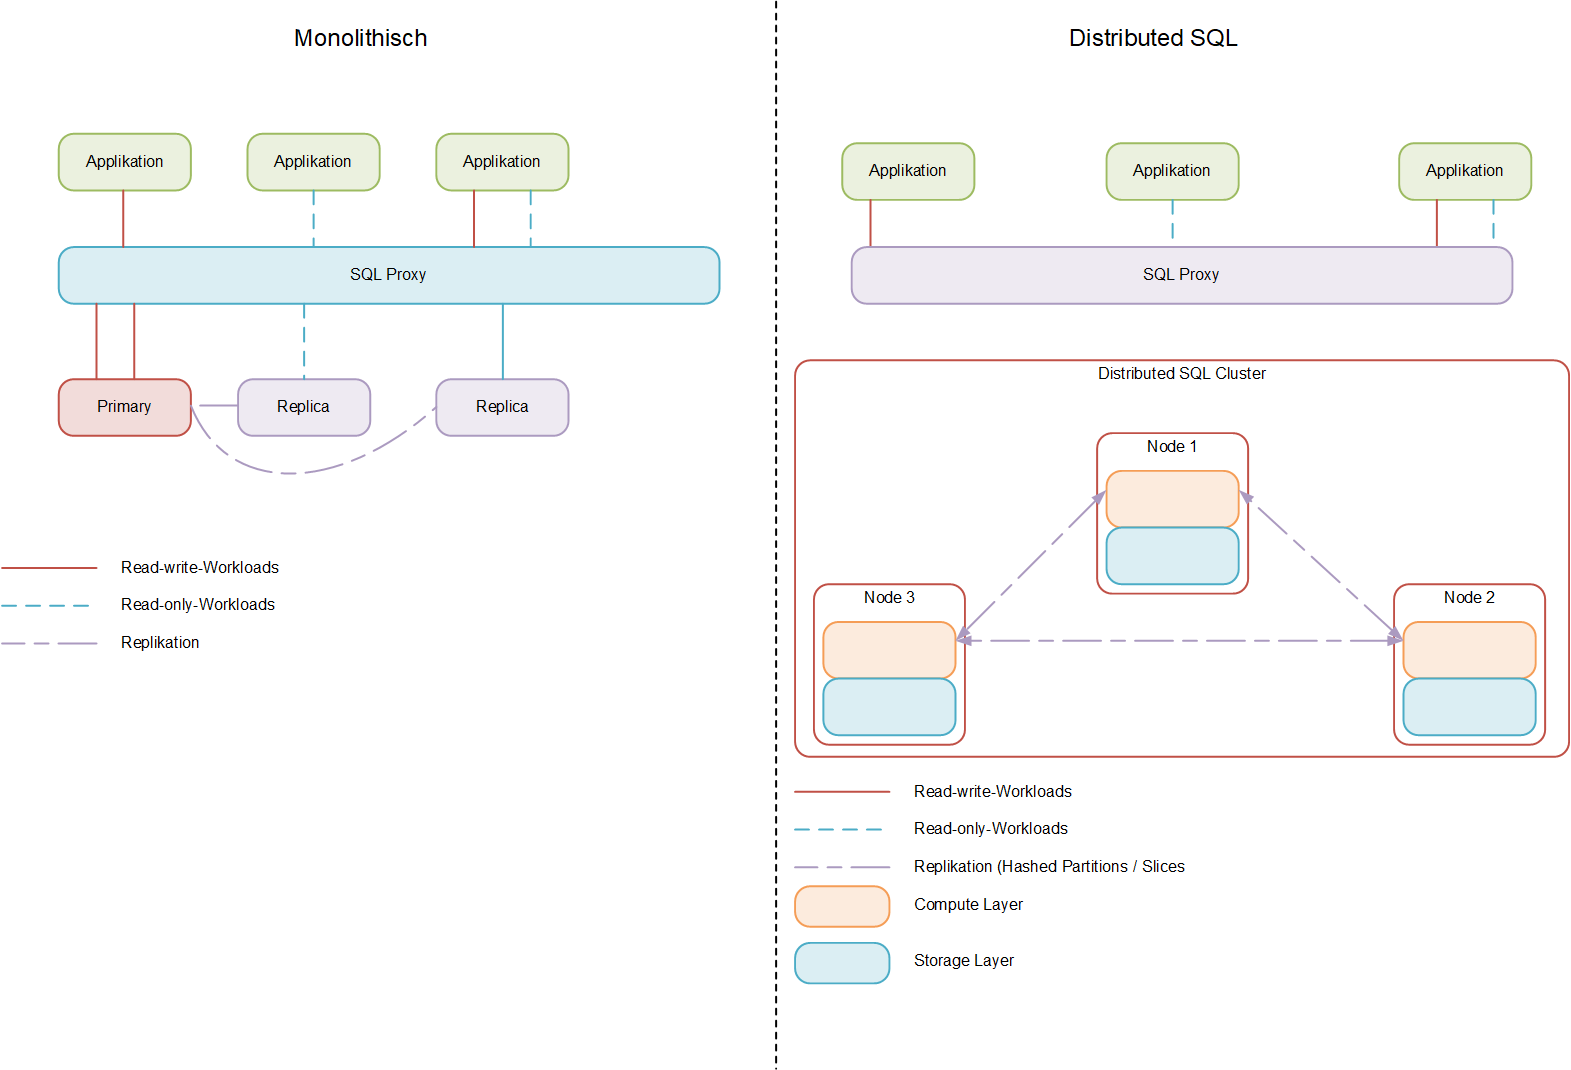
\includegraphics[width=1\linewidth]{source/implementation/evaluation/excursus_architecture/monolith_distributed}
        \caption{Monolithische vs. verteilte SQL Systeme}
        \label{fig:Monolith_vs_Distributed_SQL}
    \end{figure}
\end{flushleft}
